\documentclass{article}
% --- PACKAGES ---
\usepackage[lyric]{songs}
\usepackage[utf8]{inputenc}
\usepackage[T1]{fontenc}
\usepackage{cochineal}
\usepackage[top=2.3cm,bottom=2.3cm,left=2.3cm,right=2.3cm]{geometry}
\usepackage[dvipsnames,table,xcdraw]{xcolor}
\usepackage{eso-pic}
\usepackage{graphicx}
\usepackage{tikz}
\usetikzlibrary{calc}
\usepackage[object=vectorian]{pgfornament}
\usepackage{fancyhdr}

%\newcommand{\SongOrnament}{%
%	\par\nointerlineskip
%	\vspace{3pt}%
%	{\centering\pgfornament[width=0.4\linewidth,color=black!60!white]{89}\par}%
%	\vspace{3pt}%
%}

% --- SONG STYLING ---
\songcolumns{2}
\columnsep=2cm
\songpos{1}
\setlength{\afterpreludeskip}{3pt}
\setlength{\versesep}{15pt plus 1pt minus 1pt}
\renewcommand\printchord[1]{{\large\sffamily\itshape\color{black!60!white}#1}}
\renewcommand{\lyricfont}{\normalfont\large}
\renewcommand{\notebgcolor}{black!13!white}
\renewcommand{\snumbgcolor}{black!20!white}
\newindex{titleidx}{titleidx}	% Adăugăm cuprins
\indexsongsas{titleidx}{\thesongnum}	% Afișează numărul cântării
\setlength{\sbarheight}{0pt}	% Delete the bar between songs

% --- COVER IMAGE COMMAND ---
\newcommand\BackgroundPic{%
	\put(0,0){%
		\parbox[b][\paperheight]{\paperwidth}{%
			\vfill
			\centering
			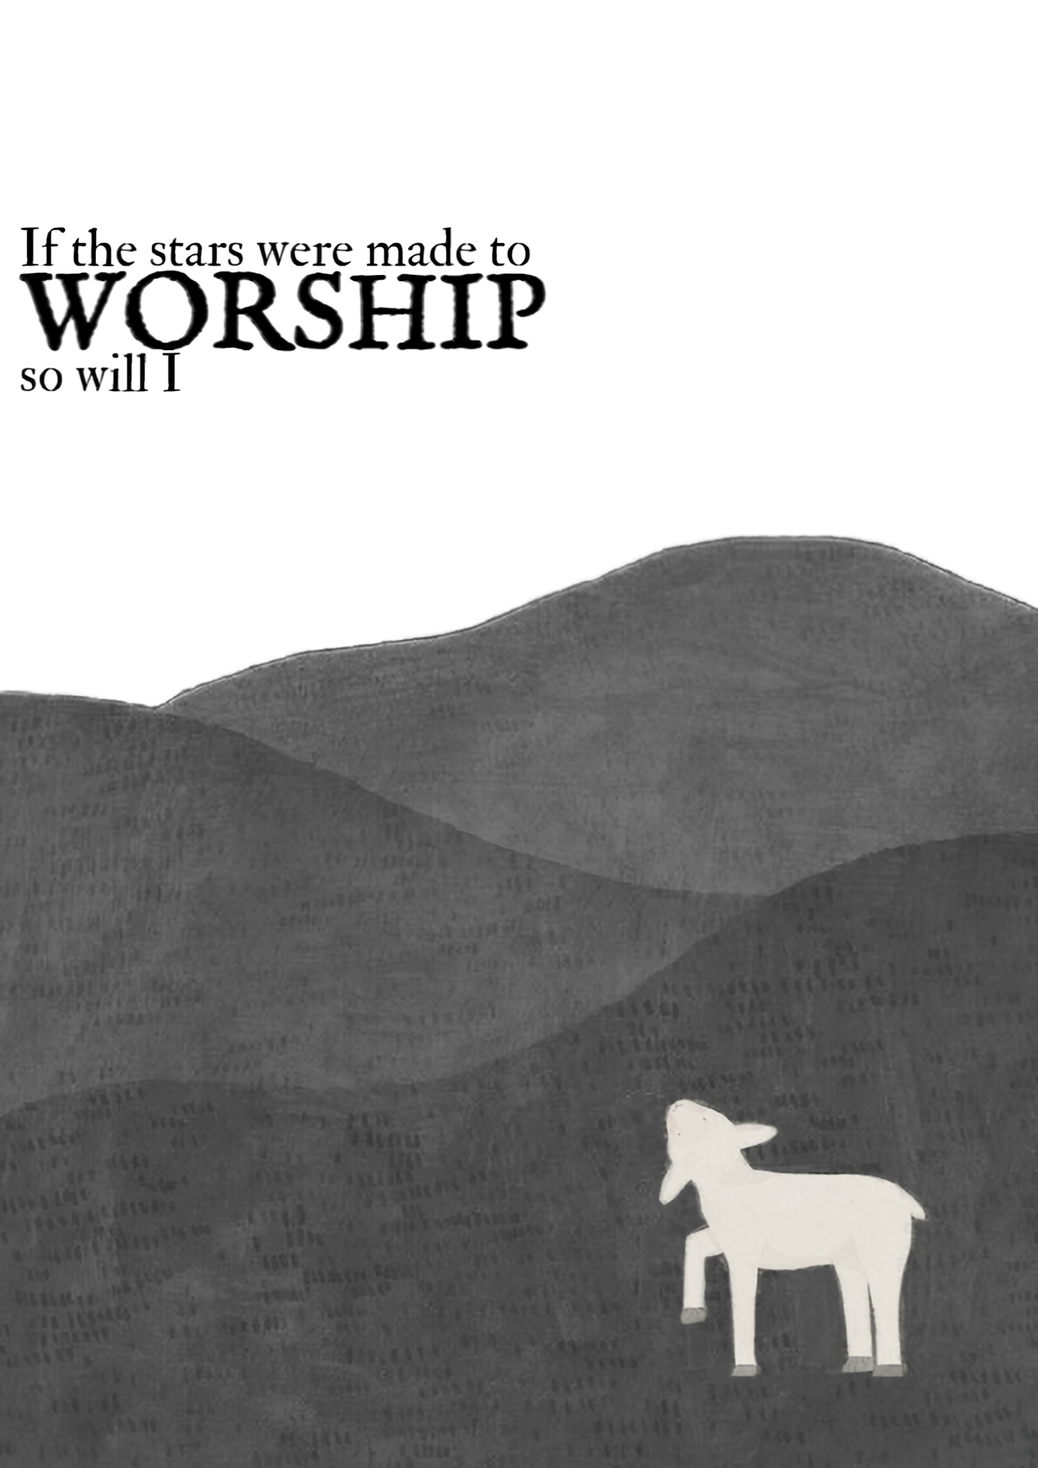
\includegraphics[width=\paperwidth]{Imagini/Copertax1_6}%
			\vfill
		}%
	}%
}

% Configure the page number footer
\pagestyle{fancy}
\fancyhf{} % Clear default headers/footers
\renewcommand{\headrulewidth}{0pt} % Remove top header line
\renewcommand{\footrulewidth}{0pt} % Remove bottom footer line

% Place the page number at the bottom center in black
\fancyfoot[C]{\small\color{black}\thepage}
\setlength{\footskip}{12pt} % Adjusts distance between lyrics and page number

% --- PAGE BORDER COMMAND (Ornament 61 + 87/89 in Chord Color) ---
\newcommand{\PageBorder}{%
	\begin{tikzpicture}[
		remember picture, 
		overlay, 
		every node/.style={inner sep=0pt}
		]
		% Se poate folosi 1 cm la shift
		% #1 pgornament pt colțuri: 61
		% #2 pgornament pt colturi: 37
		% #3 pgornament pt colturi: 41
		% #4 pgornament pt colturi: 63
		% Colțul Stânga-Sus
		\node[shift={(0.5cm,-0.5cm)},anchor=north west](CNW)	
		at (current page.north west) {\pgfornament[width=1.5cm,color=black!60!white]{41}};
		
		% Colțul Dreapta-Sus (oglindit pe verticală)
		\node[shift={(-0.5cm,-0.5cm)},anchor=north east](CNE)
		at (current page.north east) {\pgfornament[width=1.5cm,symmetry=v,color=black!60!white]{41}};
		
		% Colțul Stânga-Jos (oglindit pe orizontală)
		\node[shift={(0.5cm,0.5cm)},anchor=south west](CSW)
		at (current page.south west) {\pgfornament[width=1.5cm,symmetry=h,color=black!60!white]{41}};
		
		% Colțul Dreapta-Jos (oglindit pe ambele axe: v și h)
		\node[shift={(-0.5cm,0.5cm)},anchor=south east](CSE)
		at (current page.south east) {\pgfornament[width=1.5cm,symmetry=v,symmetry=h,color=black!60!white]{41}};
		
		% Varianta 1
		% Liniile orizontale (Sus și Jos)
		%\pgfornamentline[color=black!60!white]{CNW.north east}{CNE.north west}{3}{87}
		%\pgfornamentline[color=black!60!white]{CSW.south east}{CSE.south west}{3}{87}
		
		% Liniile verticale (Stânga și Dreapta - corectat punctul final din dreapta jos!)
		%\pgfornamentline[color=black!60!white]{CNW.south west}{CSW.north west}{4}{87}
		%\pgfornamentline[color=black!60!white]{CNE.south east}{CSE.north east}{4}{87}
		
		% Varianta 2
		% Liniile orizontale (Sus și Jos)
		\pgfornamentline[color=black!60!white]{CNW.north east}{CNE.north west}{3}{88}
		\pgfornamentline[color=black!60!white]{CSW.south east}{CSE.south west}{3}{88}
		
		% Liniile verticale (Stânga și Dreapta - corectat punctul final din dreapta jos!)
		\pgfornamentline[color=black!60!white]{CNW.south west}{CSW.north west}{4}{88}
		\pgfornamentline[color=black!60!white]{CNE.south east}{CSE.north east}{4}{88}
	\end{tikzpicture}%
}

\begin{document}
	
	% --- COVER PAGE ---
	\thispagestyle{empty}
	\AddToShipoutPictureBG*{\BackgroundPic}
	\null
	\clearpage

	% Page numbering
	\setcounter{page}{1}
	
	% --- BORDERS & SONGS ---
	\AddToShipoutPictureBG{\PageBorder}
	
	\begin{songs}{titleidx}
		
		% ----- A -----
		\input{cantari/A/A_lui_Isus_venire}
		\input{cantari/A/Aceasta_mi-e_dorinta}
		\input{cantari/A/Acum_cat_inca_se_mai_poate}
		\input{cantari/A/Acum_paraseste_acum}
		\input{cantari/A/Ai_deschis_cerul_Tau}
		\input{cantari/A/Ai_fost_mereu_de_partea_mea}
		\input{cantari/A/Ai_fost_rastignit}
		\input{cantari/A/Ai_platit_un_pret}
		\input{cantari/A/Al_Tau_e_sufletul_meu}
		\input{cantari/A/Alaturi_de_Tine}
		\input{cantari/A/Aleluia_aleluia}
		\input{cantari/A/Am_ales_pe_Domnul_Isus}
		\input{cantari/A/Am_camin_mai_sus_de_nori}
		\input{cantari/A/Am_fost_rob_dar_Isus_m-a_eliberat}
		\input{cantari/A/Am_gasit_in_Domnul_fericirea}
		\input{cantari/A/Am_gresit_de_atatea_ori}
		\input{cantari/A/Am_luat_hotararea}
		\input{cantari/A/Am_venit_din_departare}
		\input{cantari/A/Apa-i_schimbat-o-n_vin}
		\input{cantari/A/Arcuri_incordate}
		\input{cantari/A/As_da_orice}
		\input{cantari/A/As_incerca_sa_spun}
		\input{cantari/A/As_vrea_sa_numar_clipele}
		\input{cantari/A/Asculta_glasul_ce_te_cheama}
		\input{cantari/A/Astazi_cant_voios_ca_Dumnezeu}
		\input{cantari/A/Astazi_este_ziua_cantareste_bine}
		\input{cantari/A/Astazi_vin_Bunule_Tata}
		\input{cantari/A/Astazi_vin_ca_fiu_ratacitor}
		\input{cantari/A/Astazi_vin_la_Tine_Domnul_meu}
		\input{cantari/A/Astazi_vin_sa-mi_plec_genunchii}
		\input{cantari/A/Atotputernic_Tata_a_toate_creator}
		\input{cantari/A/Atunci_cand_David_lauda}
		\input{cantari/A/Azi_Domnul_este_Pastorul_meu}
		\input{cantari/A/Azi_vin_acasa_rob_nu_fiu}
		
		% ----- B -----
		\input{cantari/B/Biblia_ma-nvata}
		\input{cantari/B/Bine_ai_venit_omule}
		\input{cantari/B/Bine-ati_venit_azi_la_altar}
		\input{cantari/B/Binecuvantam_Doamne_Numele_Tau}
		\input{cantari/B/Bunatatile_Domnului_nu_se_sfarsesc}
		
		% ----- C -----
		
		\input{cantari/C/Ca_un_cerb_ce_doreste_sa_bea}
		\input{cantari/C/Ca_un_cerb_setos_de_ape}
		\input{cantari/C/Caci_un_copil_ni_s-a_nascut}
		\input{cantari/C/Calatoresc_prin_lume}
		\input{cantari/C/Cand_ajungi_sa-ti_fii_tu_insuti_o_povara}
		\input{cantari/C/Cand_eram_ratacit}
		\input{cantari/C/Cand_esti_langa_mine}
		\input{cantari/C/Cand_eu_am_aruncat_cu_pietre}
		\input{cantari/C/Cand_frigul_patrunde_in_suflet}
		\input{cantari/C/Cand_in_zare_se_iveste}
		\input{cantari/C/Cand_inalt_laude_spre_Tronul_Sfant}
		\input{cantari/C/Cand_inca_nu_eram}
		\input{cantari/C/Cand_incercarile}
		\input{cantari/C/Cand_lupta_se-apropie}
		\input{cantari/C/Cand_ma_aflu-n_prezenta_Ta}
		\input{cantari/C/Cand_ma_tem_ca_voi_cadea}
		\input{cantari/C/Cand_nici_nu_existam}
		\input{cantari/C/Cand_pe_marea_vietii_eu}
		\input{cantari/C/Cand_privesc_bolta_instelata}
		\input{cantari/C/Cand_problemele_vietii_m-apasa}
		\input{cantari/C/Cand_se_prabuseste-n_jurul_meu}
		\input{cantari/C/Cand_soarele_pe_cer_s-a_ivit}
		\input{cantari/C/Cand_sunt_cazut_si_sufletul_imi_plange}
		\input{cantari/C/Cand_sunt_rapus}
		\input{cantari/C/Cand_te_uiti_prea_mult_in_soare}
		\input{cantari/C/Cand_toti_prietenii_ma_parasesc}
		\input{cantari/C/Cand_trecem_prin_ispite_grele}
		\input{cantari/C/Cand_viata_vei_sfarsi}
		\input{cantari/C/Cand_zorii_se-arata_zambind_dimineata}
		\input{cantari/C/Cant_plin_de_bucurie}
		\input{cantari/C/Canta_suflet_al_meu}
		\input{cantari/C/Cat_de_mare_esti_Tu}
		\input{cantari/C/Cat_va_fi_pamantul}
		\input{cantari/C/Ce_bucurie_sa_ma_stiu_copilul_Tau}
		\input{cantari/C/Ce_dragoste_mare-ce_tot_a_iertat}
		\input{cantari/C/Ce_mare_esti_Tu}
		\input{cantari/C/Ce_minunat_e_sa_fii_intr-o_familie}
		\input{cantari/C/Ce_minunat_si_ce_frumos}
		\input{cantari/C/Ce_mult_astept_aceea_zi}
		\input{cantari/C/Ce_mult_Te_doresc_o_Isuse}
		\input{cantari/C/Ce_nume_minunat}
		\input{cantari/C/Cerul_declara_gloria}
		\input{cantari/C/Cerul_e-un_loc_minunat}
		\input{cantari/C/Cerul_si_pamantul}
		\input{cantari/C/Cerul_si_pamantul_ne_spune_Cuvantul}
		\input{cantari/C/Chiar_daca_grijile_te_apasa}
		\input{cantari/C/Chiar_si-n_incercare}
		\input{cantari/C/Cine_a_crezut_in_ce_ni_se_vestise}
		\input{cantari/C/Cine_sunt}
		\input{cantari/C/Cineva_se-ngrijeste}
		\input{cantari/C/Condu_pasii_mei}
		\input{cantari/C/Condu-ma_Doamne_ziua}
		\input{cantari/C/Constient_sunt_Doamne}
		\input{cantari/C/Cred_in_Domnul_Isus}
		\input{cantari/C/Cred_in_Dumnezeu_ca_Tata}
		\input{cantari/C/Credinta_noastra_mereu_neclintita}
		\input{cantari/C/Cu_gandul_la_viata_eterna}
		\input{cantari/C/Cu_imnuri_de_marire}
		\input{cantari/C/Cu_mult_in_urma-n_Betleem}
		\input{cantari/C/Cu_Tine_drag_Isuse}
		\input{cantari/C/Cu_Tine_nu_sunt_singur}
		\input{cantari/C/Cu_Tine-n_gand}
		\input{cantari/C/Cu-a_Ta_iubire_si_indurare}
		\input{cantari/C/Cum_as_putea_sa_tac}
		\input{cantari/C/Cum_doreste_un_cerb}
		\input{cantari/C/Cum_pot_rasplati_eu}
		\input{cantari/C/Cum_sa_nu_Te_cant_Isuse}
		\input{cantari/C/Cu-ndurare_El_m-a_ridicat}
		
	\end{songs}
	
	\clearpage
	\begin{center}
		{\Huge\bfseries Cuprins Alfabetic}
	\end{center}
	\begin{multicols}{2}
		\input{titleidx.sbx}
	\end{multicols}
	%\showindex[2]{Cuprins}{titleidx}	% Afișează cuprinsul în 2 coloane
	% Pentru compilarea indexului: Tools -> External Terminal -> 
	% _{songidx titleidx.sxd titleidx.sbx}
	
\end{document}